\documentclass[12pt,a4paper]{report}
\usepackage[utf8]{inputenc}
\usepackage[spanish]{babel}
\usepackage{amsmath}
\usepackage{amsfonts}
\usepackage{amssymb}
\usepackage{graphicx}
\usepackage[left=2cm,right=2cm,top=2cm,bottom=2cm]{geometry}
\author{Oscar Cruz Cervantes}

\begin{document}
\begin{center}
Practica 7\\
Sistemas electronicos de interfaz\\
Oscar Cruz Cervantes 18311638\\

\includegraphics[scale=1.5]{01.png}\\
Ingenieria Mecatronica\\
\end{center}

\newpage
\section{objetivo}
Hacer uso del transistor Darlintong y del LDR\\
\section{Materiales}
1- Protoboard\\
2- LDR\\
3- Cables para proto\\
4- Tip 112\\
5- Resitencias varias\\
6- Diodo de acciòn rapida\\
7- LED
\section{Procedimiento}
Primero deberemos simular el diagrama que nos fue dado por el profesor.\\
\begin{center}
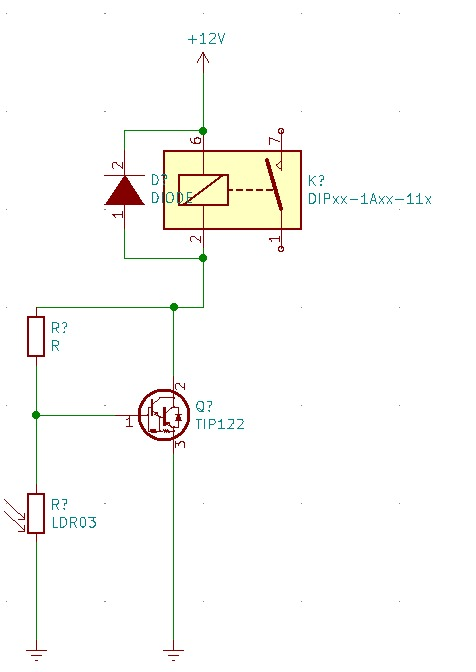
\includegraphics[scale=0.5]{02.jpeg}\\
\end{center}
Esto con la finalidad de verificar el funcionamiento del circuito y encontrar el tamaño de la resitencia. Despùes comenzaremos con el armado del circuito, en este circuito yo utilice un potenciometro para evitar buscar la resistencia necesaria facilitando el armado de este ya que la resistencia que se nos habia indicado era muy alta.

\section{Conclusiòn}
Esta practi fue un poco complicada ya que desconocia el funcionamiento del LDR y ademàs las resistencias que se nos habian indicado no servia para este circuito, pero una vez comprendido el funcionamiento y usos del LDR el lograr que este funcione es muy sencillo, ademàs si usas un potenciometro es myu sensillo encontrar la resistencia para este sircuito ya que solo tienes que hacerlo funcionar y despues mides la ressistencia del potenciometro.\\
\begin{center}
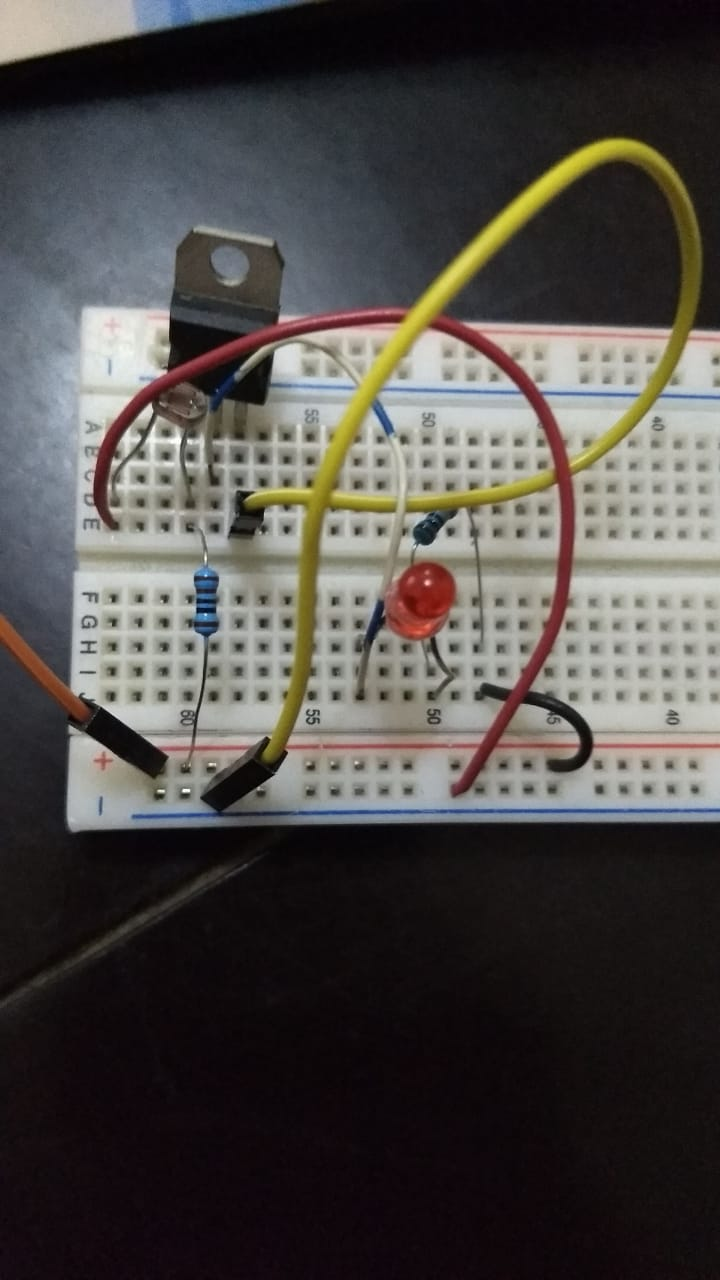
\includegraphics[scale=.4]{LDR.jpeg}
\end{center}

\end{document}